% 3456789012345678901234567890123456789012345678901234567890123456789012
%        1         2         3         4         5         6         7
%
% Format: LaTeX
%
% For information about this file, contact the author by email at
% joe.loughry@stx.ox.ac.uk, or by telephone: +44 (0)7984147430 (mobile),
% or +1 303 221 4380 (office).  The time zone is GMT minus 7 hours.
%

\documentclass{beamer}

\usepackage{url}
\usepackage{hyperref}

%
% end of preamble
%

\title{A Model of Certifier and Accreditor Risk Calculation for Multi-Level Systems}
\author{Joe Loughry \\
	\url{mailto:joe.loughry@stx.ox.ac.uk}}

\institute{Department of Computer Science, University of Oxford \\
	Wolfson Building, Parks Road, Oxford, OX1 3QD, UK}
\date{IEEE HST'13 \\ Boston, 12--14 Nov.\ 2013}

\begin{document}

\begin{frame}
	\titlepage
	\vfill
	{\tiny Build \input{slides_build_counter.txt}}
\end{frame}

\begin{frame}
	\frametitle{Topics}
	\begin{enumerate}
		\item C\&A in 60 Seconds
		\item Where all this data came from
		\item Findings
		\item Summary and Conclusion
	\end{enumerate}
\end{frame}

\begin{frame}
	\frametitle{C\&A in 60 Seconds}
	\begin{center}
		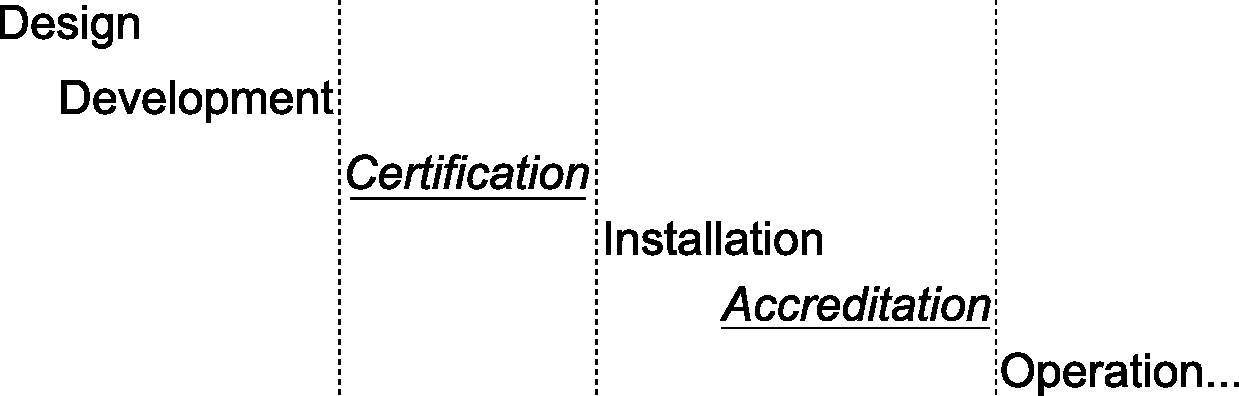
\includegraphics[width=\textwidth]{waterfall_drawing_for_slides.pdf}
	\end{center}
\end{frame}

\begin{frame}
	\frametitle{Where this data came from}
	\begin{itemize}
		\item Grateful acknowledgement is given to Lockheed Martin
			for access to project records and data:
			\begin{itemize}
				\item \ldots from an unsuccessful Common Criteria (CC) security
					evaluation in 2006
				\item \ldots and from the \emph{successful} DIACAP security
					certification of a similar product in 2010
				\item \ldots as well as from a previous CC validation of an
					earlier version of the same product in 1999.
			\end{itemize}
		\item Methodology: participant observation, grounded theory.
	\end{itemize}
\end{frame}

% Notes: my methodology was participant observation. Anonymisation of sources.
% Use of grounded theory.

\begin{frame}
	\frametitle{Findings}
	\begin{itemize}
		\item Certifier model (observational)
		\item Accreditor model (analytical)
		\item Grounded theory of implicit and explicit communication channels in C\&A
		\item Proof that channels exist and are reliable
		\item Paradox in security rules
	\end{itemize}
	\vfill
	Assumptions, applicability, and practical applications.
\end{frame}

\begin{frame}
	\frametitle{Assumptions}
	\begin{enumerate}
		\item Accreditors have appropriate security clearances for their jobs.
		\item Every cross domain system has exactly $n=2$ accreditors.
	\end{enumerate}
\end{frame}

\begin{frame}
	\frametitle{This is Accreditor \#1's view of the situation.}
	\begin{center}
		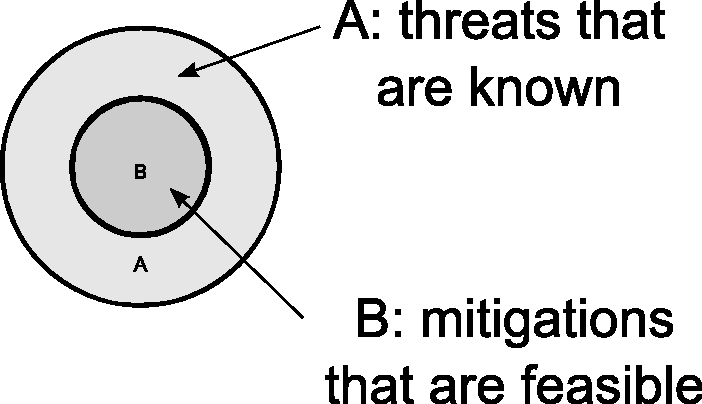
\includegraphics[width=\textwidth]{venn_diagrams_for_slides_1.pdf}
	\end{center}
\end{frame}

\begin{frame}
	\frametitle{Accreditor \#2 has a different, equally valid perspective.}
	\begin{center}
		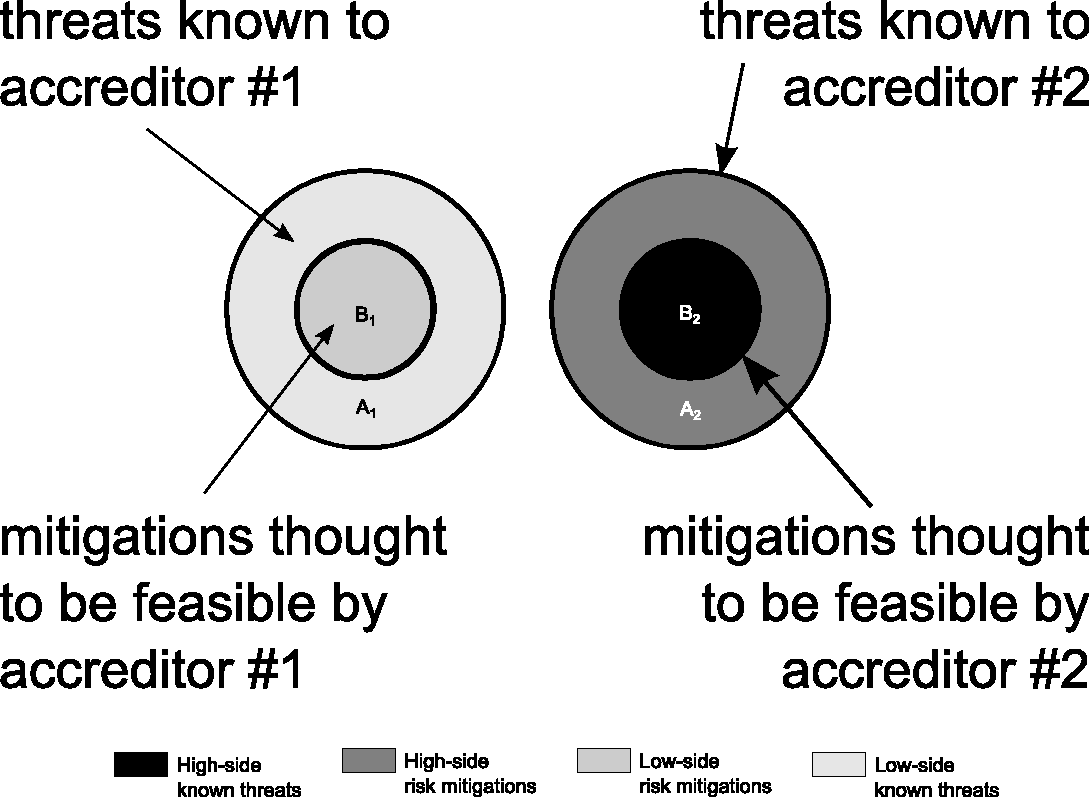
\includegraphics[width=\textwidth]{venn_diagrams_for_slides_2.pdf}
	\end{center}
\end{frame}

\begin{frame}
	\frametitle{Public information}
	\begin{center}
		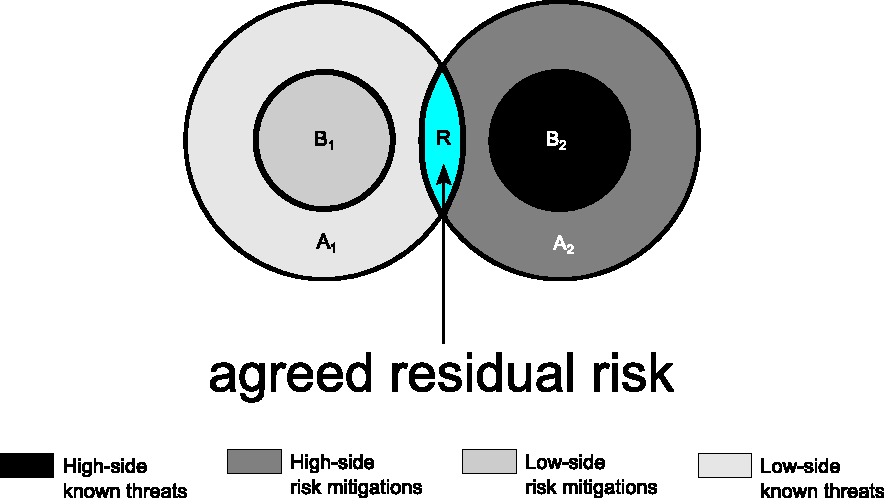
\includegraphics[width=\textwidth]{venn_diagrams_for_slides_3.pdf}
	\end{center}
\end{frame}

\begin{frame}
	\frametitle{Classified information with risk of information leakage}
	\begin{center}
		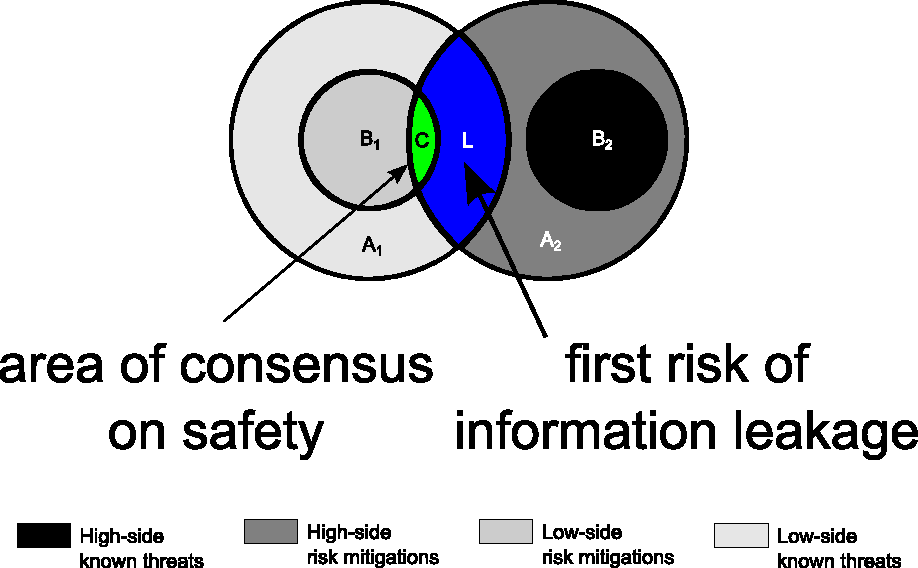
\includegraphics[width=\textwidth]{venn_diagrams_for_slides_4.pdf}
	\end{center}
\end{frame}

\begin{frame}
	\frametitle{Personal risk to Accreditor \#2}
	\begin{center}
		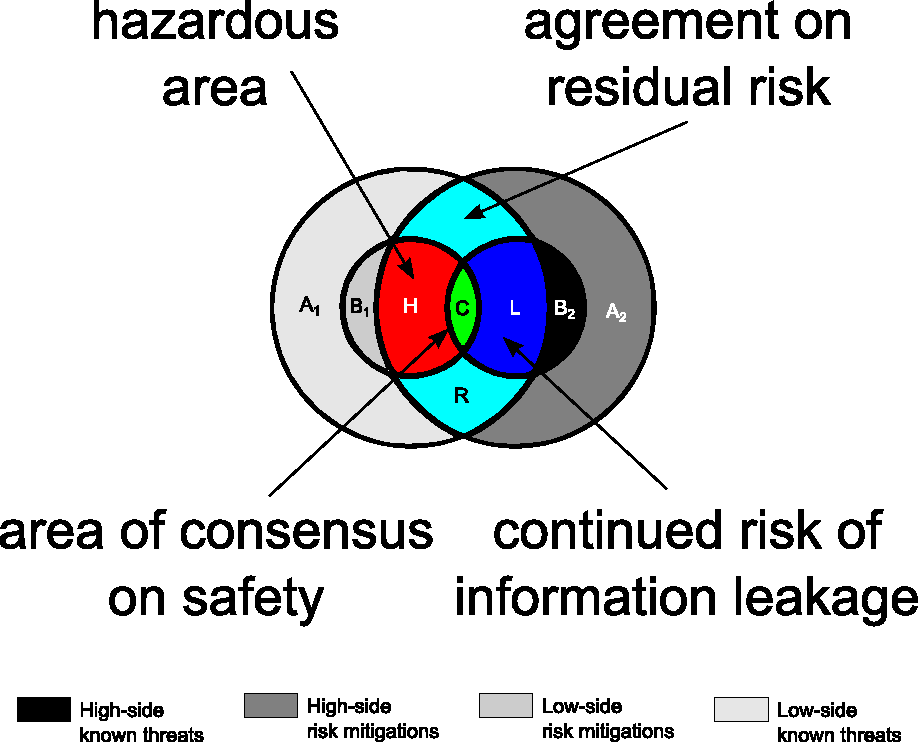
\includegraphics[width=\textwidth]{venn_diagrams_for_slides_5.pdf}
	\end{center}
\end{frame}

\begin{frame}
	\frametitle{As the situation approaches a pure collateral\ldots}
	\begin{center}
		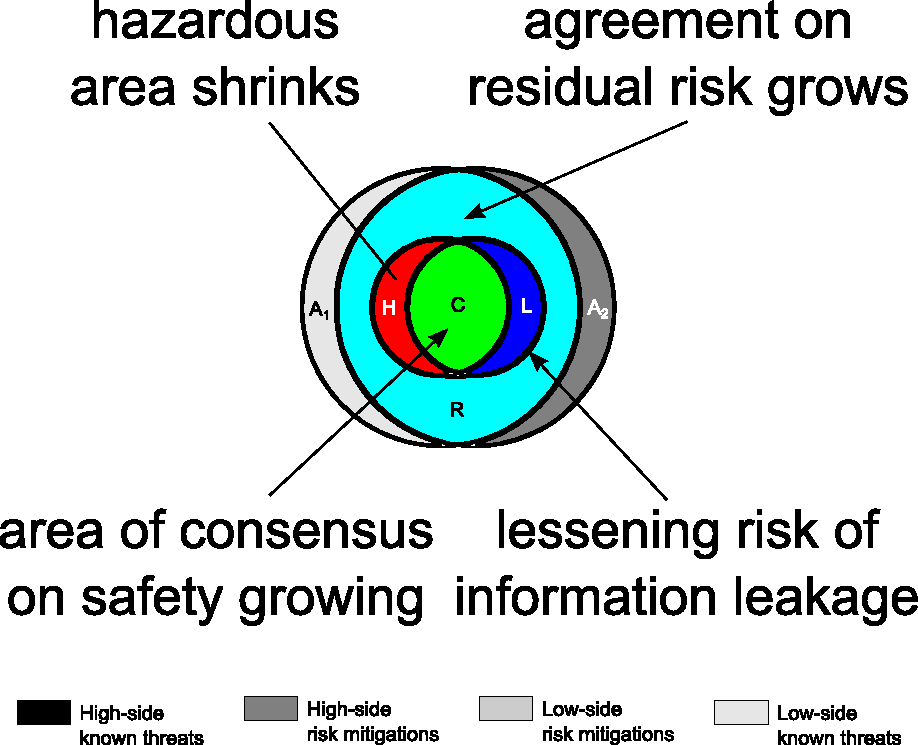
\includegraphics[width=\textwidth]{venn_diagrams_for_slides_6.pdf}
	\end{center}
\end{frame}

\begin{frame}
	\frametitle{\ldots degenerate situation\ldots}
	\begin{center}
		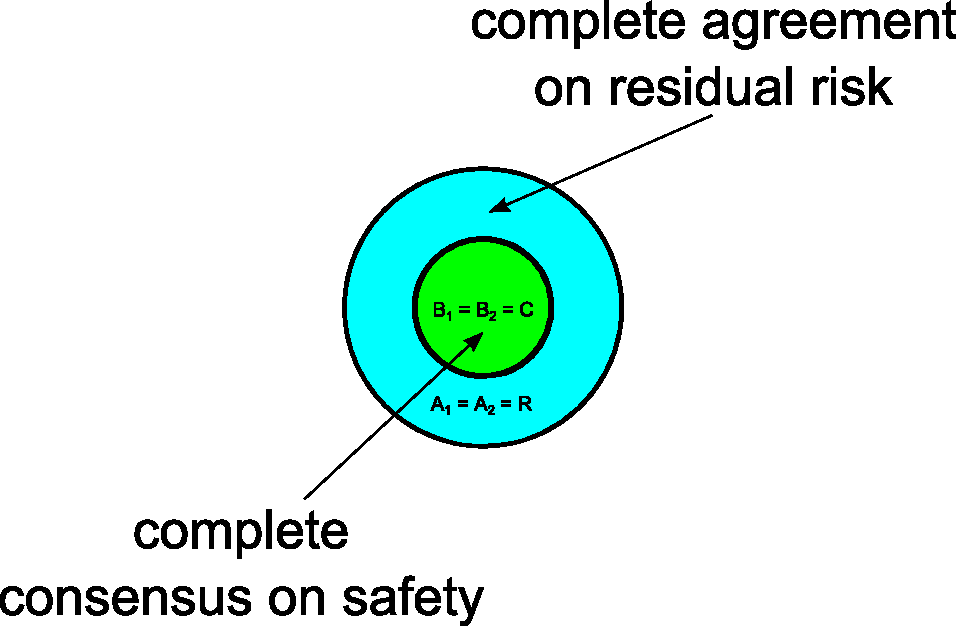
\includegraphics[width=\textwidth]{venn_diagrams_for_slides_7.pdf}
	\end{center}
\end{frame}

\begin{frame}
	\frametitle{Collateral with different security clearances}
	\begin{center}
		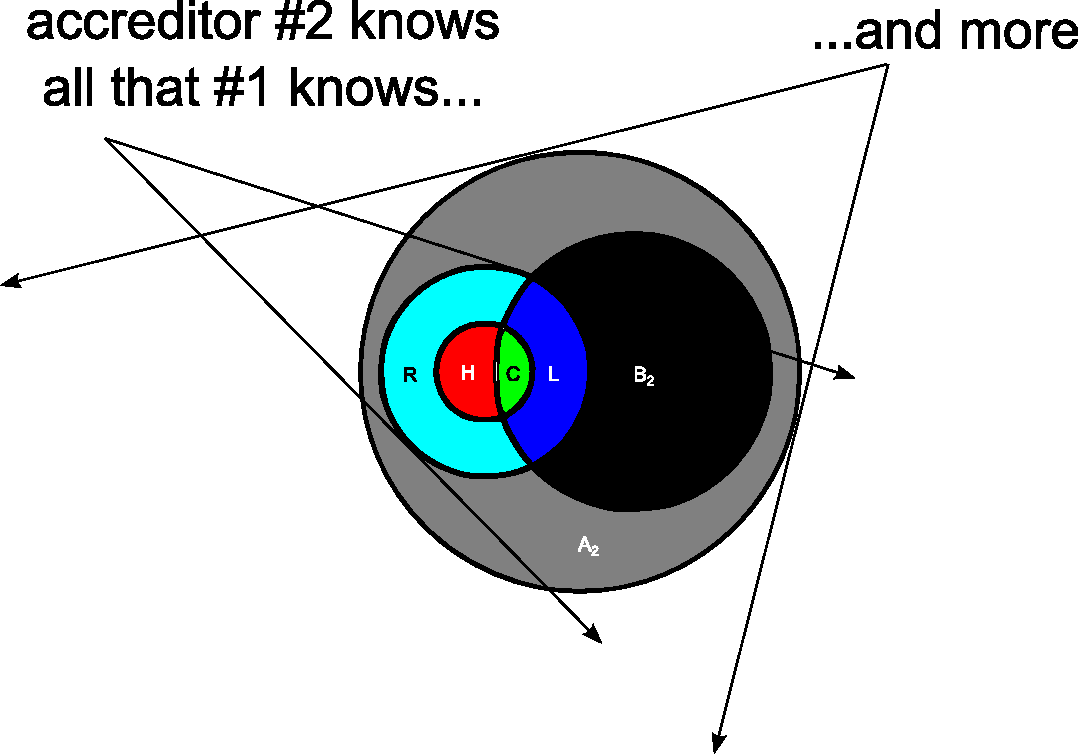
\includegraphics[width=\textwidth]{venn_diagrams_for_slides_8.pdf}
	\end{center}
\end{frame}

\begin{frame}
	\frametitle{Security paradox!}
	\begin{center}
		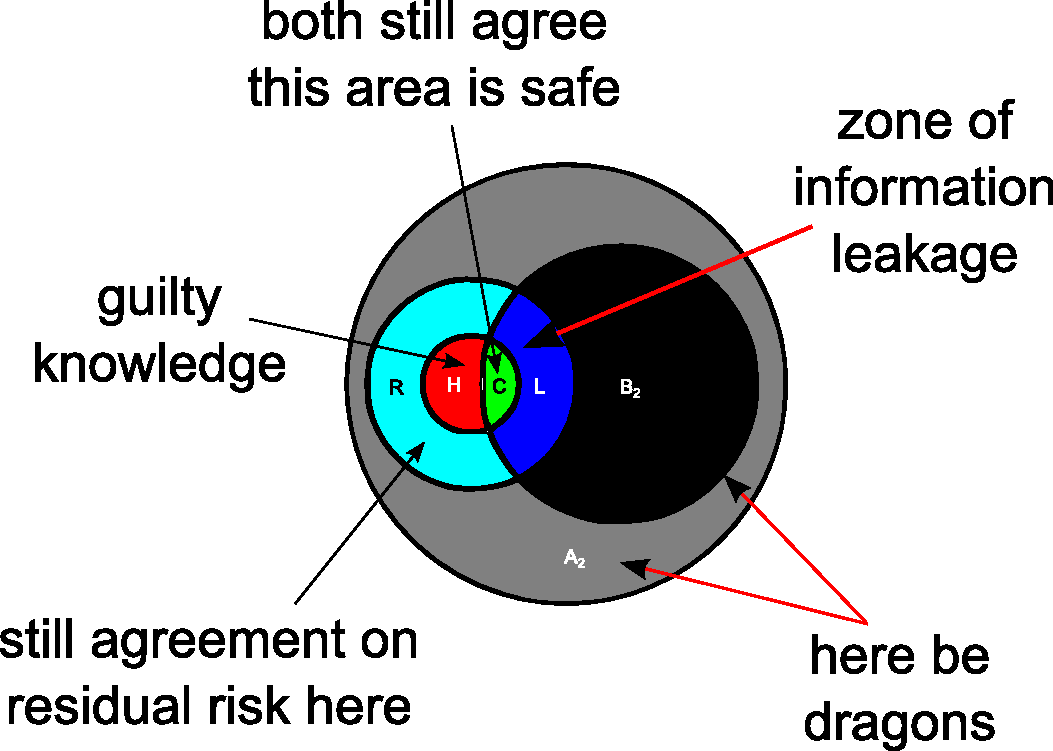
\includegraphics[width=\textwidth]{venn_diagrams_for_slides_9.pdf}
	\end{center}
\end{frame}

\begin{frame}
	\frametitle{Summary and Conclusion}
	\begin{enumerate}
		\item Some desirable information flows are inhibited by security policy.
		\item Some \emph{undesirable} information flows are forced.
		\item The paradox of looser security rules.
		\item It is possible, within limits, to predict the duration of accreditation.
		\item Developer can exert a measure of control over certification schedule.
	\end{enumerate}
\end{frame}

\begin{frame}
	\begin{center}
		\vspace{1cm}
		% trim is left, bottom, right, top of a US-letter page for this particular graphic.
		
\includegraphics[width=0.3\textwidth,trim=0 0 117mm 183mm,clip]{ox_brand_cmyk_pos.pdf}
		\vfill
		\url{mailto:joe.loughry@stx.ox.ac.uk}
	\end{center}
\end{frame}

\end{document}

